% LaTeX test 
\documentclass[a4paper,11pt,fleqn]{article}

\usepackage{kotex}
\usepackage{amssymb}
\usepackage{gensymb}
\usepackage{color}
\usepackage{graphicx}
\DeclareGraphicsExtensions{.pdf,.png,.jpg}

\usepackage{amsmath}
\usepackage{hyperref}

\usepackage{fancyhdr}
\pagestyle{fancy}
\lhead{ds4dqs@gsa.hs.kr} 
\chead{} 
\rhead{Gwangju Science Academy for the gifted}
\lfoot{} 
\cfoot{} 
\rfoot{\today}

\usepackage{verbatim}
\usepackage{enumitem}

\newcommand{\n}{\newline}

\begin{document}
\textcolor{blue}{mid term exam.} \n
\rule{\linewidth}{1pt}
\n
답안  \n 
\rule{\linewidth}{0.8pt}
.
\n
%\item
최용석
\n
\begin{eqnarray*}
	\vec{L} &=& \sum_i ( \vec{r}_{cm} + \vec{r_i }' ) \times m_i ( \vec{v}_{cm} + \vec{v_i }')\\
	&=& \sum_i ( \vec{r}_{cm} \times m_i \vec{v}_{cm}) + \sum_i ( \vec{r}_{cm} \times m_i \vec{v_i}')
	+ \sum_i ( \vec{r_i}' \times m_i \vec{v}_{cm} ) + \sum_i ( \vec{r_i}' \times m_i \vec{v_i}')\\
	&=& \vec{r}_{cm} \times \left( \sum_i m_i \right) \vec{v}_{cm} + \vec{r}_{cm}\times \sum_i m_i \vec{v_i}' 
	+ \left( \sum_i m_i \vec{r_i}' \right) \times \vec{v}_{cm} + \sum_i ( \vec{r_i}' \times m_i \vec{v_i}')
\end{eqnarray*}
\[
	\sum_i m_i \vec{r_i}' = \sum_i m_i ( \vec{r_i} - \vec{r}_{cm} ) = \sum_i m_i \vec{r_i} - m \vec{r}_{cm} = 0
\]
\[
	\sum_i m_i \vec{v_i}' = \sum_i m_i \vec{v_i} - m \vec{v}_{cm} = 0
\]
\[
	\vec{L} = \vec{r}_{cm} \times m \vec{v}_{cm} + \sum_i \vec{r_i}' \times m_i \vec{v_i}'
\]





\begin{enumerate}[start=12]
%%%%%%%%%%%%%%%%%%%%%%%%%%%%%%%%%%%%%%%%%%%%%%%%%%%% 12
\item
	\[
		I_1 = \frac{1}{12} M a^2
	\]
	\[
		I_2 = \frac{1}{12} M b^2
	\]
	\[
		I_3 = \frac{1}{12} M (a^2 + b^2)
	\]
\n


%%%%%%%%%%%%%%%%%%%%%%%%%%%%%%%%%%%%%%%%%%%%%%%%%%%% 13
\newpage
\item 
.\n

\[
	\vec{L} = \sum_i m_i ( \vec{r_i} \times \vec{v_i} ) = \sum_i \{ \vec{r_i} \times ( \vec{\omega} \times \vec{r_i} ) \}
\]
\[
	\vec{\omega} \times \vec{r_1} = \begin{pmatrix} \hat{i} & \hat{j} & \hat{j} \\ 3 & -2 & 4 \\ 1 & -1 & 1 \end{pmatrix} = 2 \hat{i} + \hat{j} - \hat{k}	
\]
\[
	\vec{r_1} \times ( \vec{\omega} \times \vec{r_1}) = \begin{pmatrix} \hat{i} & \hat{j} & \hat{j} \\ 1 & -1 & 1 \\ 2 & 1 & -1 \end{pmatrix} = 3 \hat{j} + 3 \hat{k}
\]

\[
\vec{\omega} \times \vec{r_2} = \begin{pmatrix} \hat{i} & \hat{j} & \hat{j} \\ 3 & -2 & 4 \\ 2 & 0 & 2 \end{pmatrix} = -4 \hat{i} + 2\hat{j} +4 \hat{k}	
\]
\[
\vec{r_2} \times ( \vec{\omega} \times \vec{r_2}) = \begin{pmatrix} \hat{i} & \hat{j} & \hat{j} \\ 2 & 0 & 2 \\ -4 & 2 & 4 \end{pmatrix} = -4 \hat{i} -16 \hat{j} + 4 \hat{k}
\]

\[
\vec{\omega} \times \vec{r_3} = \begin{pmatrix} \hat{i} & \hat{j} & \hat{j} \\ 3 & -2 & 4 \\ -1 & 1 & 0 \end{pmatrix} = -4 \hat{i} -4 \hat{j} + \hat{k}	
\]
\[
\vec{r_3} \times ( \vec{\omega} \times \vec{r_3}) = \begin{pmatrix} \hat{i} & \hat{j} & \hat{j} \\ -1 & 1 & 0 \\ -4 & -4 & 1 \end{pmatrix} = \hat{i} + \hat{j} + 8 \hat{k}
\]

\[
	\vec{L} = ( -4 +4 ) \hat{i} + ( 6 -16 +4 ) \hat{j} + ( 6 + 4 + 32 ) \hat{k} = -6 \hat{j} + 42 \hat{k}
\]
\n


%%%%%%%%%%%%%%%%%%%%%%%%%%%%%%%%%%%%%%%%%%%%%%%%%%%% 14
\newpage
\item
\begin{eqnarray*}
	I_{xx} &=& \sum_i m_i ( y_i^2 + z_i ^2 ) \\
	&=& 2(1+1) + 1(0+4) + 4(1+0) \\
	&=& 12
\end{eqnarray*}
\begin{eqnarray*}
	I_{yy} &=& \sum_i m_i ( z_i^2 + x_i ^2 ) \\
	&=& 2(1+1) + 1(4+4) + 4(0+1) \\
	&=& 16
\end{eqnarray*}
\begin{eqnarray*}
	I_{zz} &=& \sum_i m_i ( x_i^2 + y_i ^2 ) \\
	&=& 2(1+1) + 1(4+0) + 4(1+1) \\
	&=& 16
\end{eqnarray*}
\begin{eqnarray*}
	I_{xy} = I_{yx} &=& - \sum_i m_i x_i y_i \\
	&=& -2(-1) - 1(0) - 4(-1) \\
	&=& 6
\end{eqnarray*}
\begin{eqnarray*}
	I_{yz} = I_{zy} &=& - \sum_i m_i y_i z_i \\
	&=& -2(-1) - 1(0) - 4(0) \\
	&=& 2
\end{eqnarray*}
\begin{eqnarray*}
	I_{zx} = I_{xz} &=& - \sum_i m_i z_i x_i \\
	&=& -2(1) - 1(4) - 4(0) \\
	&=& -6
\end{eqnarray*}
\[
\tilde{I} = \begin{pmatrix}
	I_{xx} & I_{xy} & I_{xz} \\
	I_{yx} & I_{yy} & I_{yz} \\
	I_{zx} & I_{zy} & I_{zz}
	\end{pmatrix} = 
	\begin{pmatrix}
		12 & 6 & -6 \\
		6 & 16 & 2 \\
		-6 & 2 & 16
	\end{pmatrix}
\]
\n\n


%%%%%%%%%%%%%%%%%%%%%%%%%%%%%%%%%%%%%%%%%%%%%%%%%%%% 15
\item 
\begin{eqnarray*}
	I_{xx} &=& \int _0 ^a \int _0 ^a \sigma ( y^2 + z^2 ) dy dz \\
	&=& \int _0 ^a \sigma \left( \frac{a^3}{3} + z^2 a \right) dz \\
	&=& \sigma \left( \frac{a^4}{3} + \frac{a^4}{3} \right) \\
	&=& \sigma a^2 \left( \frac{2}{3} a^2 \right) \\
	&=& \frac{2}{3} M a^2 \\
	&=& I_{yy} \\
	&=& I_{zz}
\end{eqnarray*}
\begin{eqnarray*}
	I_{xy} &=& - \int _0 ^a \int _0 ^a \sigma xy dx dy \\
	&=& - \sigma \int _0 ^a \frac{a^2}{2} y dy \\
	&=& - \sigma \frac{a^4}{4} \\
	&=& - \frac{1}{4} M a^2 \\
	&=& I_{yz} \\
	&=& I_{zx}
\end{eqnarray*}
\n\n

\newpage
%%%%%%%%%%%%%%%%%%%%%%%%%%%%%%%%%%%%%%%%%%%%%%%%%%%% 16
\item
(a) \n\n
\begin{eqnarray*}
	\vec{L} &=& \tilde{I} \vec{\omega} = Ma^2 \begin{pmatrix}
		\frac{2}{3} & -\frac{1}{4} & -\frac{1}{4} \\
		-\frac{1}{4} & \frac{2}{3} & -\frac{1}{4} \\
		-\frac{1}{4} & -\frac{1}{4} & \frac{2}{3}
	\end{pmatrix} \begin{pmatrix}
	2 \\ 5 \\ -3 \end{pmatrix} \\
	&=& \frac{1}{12} M a^2 \begin{pmatrix}
		8 & -3 & -3 \\
		-3 & 8 & -3 \\
		-3 & -3 & 8 \end{pmatrix} \begin{pmatrix}
		2 \\ 5 \\ -3
	\end{pmatrix} \\
	&=& \frac{1}{12} M a^2 \begin{pmatrix}
		10 \\ 43 \\ -45
	\end{pmatrix} \\
	&=& \frac{1}{12} M a^2 ( 10 \hat{i} + 43 \hat{j} -45 \hat{k})
\end{eqnarray*}
\n
(b) \n\n
\begin{eqnarray*}
	T_{rot} &=& \frac{1}{2} \tilde{\vec{\omega}} \tilde{I} \vec{\omega} \\
	&=& \frac{1}{2} \begin{pmatrix}
		2 & 5 & -3
	\end{pmatrix} \begin{pmatrix}
	8 & -3 & -3 \\
	-3 & 8 & -3 \\
	-3 & -3 & 8 \end{pmatrix} \begin{pmatrix}
	2\\5\\-3
	\end{pmatrix} \frac{1}{12} M a^2 \\
	&=& \frac{1}{24} M a^2 \begin{pmatrix}
		10 & 43 & -45
	\end{pmatrix} \begin{pmatrix}
	2\\5\\-3 \end{pmatrix} \\
	&=& \frac{1}{24} M a^2 ( 20 + 215 + 135) \\
	&=& \frac{185}{12} M a^2
\end{eqnarray*}
\n\n\n\n\n\n\n\n


%%%%%%%%%%%%%%%%%%%%%%%%%%%%%%%%%%%%%%%%%%%%%%%%%%%% 17
\newpage
\item
질량중심으로부터 거리는 각각 그림과 같다.
\begin{figure}[h]
	\begin{center}
		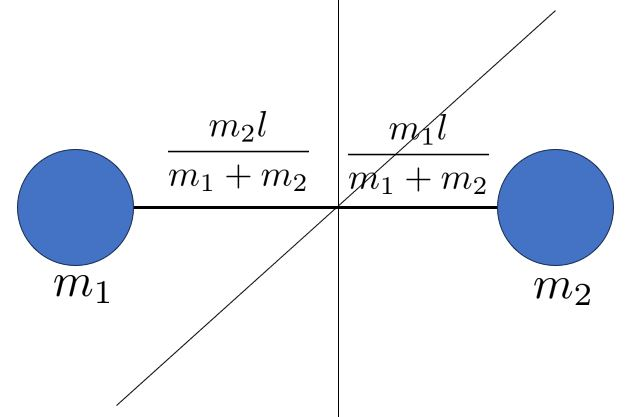
\includegraphics[scale=0.5]{img/dumbell}
		%\caption{캡션} \label{fig:label}
	\end{center}
\end{figure}
\n
\begin{eqnarray*}
	I_1 &=& m_1 \cdot \left( \frac{m_2 l}{m_1 + m_2} \right) ^2 + m_2 \cdot \left( \frac{m_1 l}{m_1 + m_2 } \right) ^2 \\
	&=& \frac{m_1 m_2 ( m_1 + m_2 )}{( m_1 + m_2 ) ^2} l^2 \\
	&=& \frac{m_1 m_2}{m_1 + m_2} l^2 \\
	&=& I_2 \\
	I_3 &=& 0
\end{eqnarray*}
\n\n\n




\end{enumerate}

\begin{comment}
\begin{displaymath}

\end{displaymath}
\begin{eqnarray*}
e^{2i \theta} &=& cos 2 \theta + i sin 2 \theta \\
( e^{i \theta} ) ^2  &=& ( cos \theta + i sin \theta ) ^2 = cos ^2 \theta - sin ^2 \theta + 2 i cos \theta sin \theta
\end{eqnarray*}
\begin{equation}
sin 3 \theta = 3sin \theta - 4 sin ^3 \theta
\end{equation}

 \begin{figure}[htbp] 옵션 here, top, bottom, page of floats
\begin{figure}[h]
\begin{center}
    \includegraphics[scale=0.9]{009}
    \caption{캡션} \label{fig:label}
\end{center}
\end{figure}

\textcolor{blue}{색깔 있는 글자}
\rule{\linewidth}{1pt}  긴 줄을 긋고 
\newline  새 줄로

\end{comment}
\end{document}
